While \PNAME can compose with other FPGA-accelerated simulators, in this paper
we extend FireSim~\cite{firesim} and {\SIMNAME}~\cite{midas}. \SIMNAME is a
compiler that generates FPGA-accelerated simulators automatically from Chisel
RTL. MIDAS is not standalone; FireSim provides a development
environment, with RTL and software models for complete target designs, as well
and powerful utilities to batch out FPGA builds and simulations across Amazon EC2.

\section{Host-Target Decoupling}\label{sec:target-decoupling}
Generally, host-target decoupling begins with a \emph{target abstraction} that
represents the target and its environment as a dataflow graph of actors~\cite{LIBDN,APortNetworks}.  The target abstraction we use in this paper
derives from the one used in RAMP~\cite{RAMP} and resembles a
synchronous-dataflow graph~\cite{SDF} where:

\begin{itemize}
    \item \emph{Tokens} are messages passed between the nodes of the graph. Tokens represent
        the values on wires in the target at the end of a target cycle.
    \item \emph{Models} are graph nodes that model the behavior of a
        synchronous block of RTL. Each model executes one target cycle of
        simulation by dequeuing a token from each of its inputs and enqueuing
        a token into each of its outputs.
    \item \emph{Channels} are the edges of graph. They transport tokens
        between models and simulate target-interconnect latency, buffering, and clock-domain crossings. At the start of simulation, a channel is initialized with
        a number of tokens equal to its latency.
\end{itemize}
%
%\begin{figure*}
%	\centering
%    \begin{subfigure}[t]{0.32\textwidth}
%        \includegraphics[width=\columnwidth]{figures/adder-example1.pdf}
%        % graffle2pdf -c initial-state midas-graphics/graffle/adder-example.graffle figures/adder-example1.pdf
%    \end{subfigure}
%    \begin{subfigure}[t]{0.32\textwidth}
%        \includegraphics[width=\columnwidth]{figures/adder-example2.pdf}
%        % graffle2pdf -c tfire-cycle0 midas-graphics/graffle/adder-example.graffle figures/adder-example2.pdf
%    \end{subfigure}
%    \begin{subfigure}[t]{0.32\textwidth}
%        \includegraphics[width=\columnwidth]{figures/adder-example3.pdf}
%        % graffle3pdf -c cycle-1 midas-graphics/graffle/adder-example.graffle figures/adder-example3.pdf
%    \end{subfigure}
%	\centering
%    \caption{A 32-bit adder and environment simulating a single cycle of target time.}
%    \label{fig:adder-example}
%\vspace{-0.1in}
%\end{figure*}
%
%Figure~\ref{fig:adder-example} illustrates an example graph, consisting of a
%single 32-bit adder unit, composed with source and sink units, as it executes
%one cycle of target time.

A simulator that faithfully implements this graph decouples target time from
host time. Unlike in an FPGA prototype, where every FPGA clock cycle emulates a
target clock cycle, an FPGA-hosted model only executes a target-clock-cycle when
it can legally fire. Thus, the behavior of the target is decoupled from the
host, allowing simulators to be partitioned across the host and to tolerate
variable-host-latencies to DRAM and the CPU, while remaining deterministic.
Unfortunately, this results in target time advancing slower than it would in an
FPGA prototype of the same host frequency.  This is quantified by the
FPGA-cycle-to-Model-cycle Ratio~(FMR)\cite{APortNetworks}, below, which increases from
one~(the simulator simulates a target cycle on every FPGA host cycle) as the simulator stalls on token availability and backpressure. The FMR
of a simulator is variable: it is a function of both application-dependent
behavior in the target and variable latencies in host services.
$$ FMR = \frac{Cycles_{FPGA}}{Cycles_{Target}}$$

\section{The \SIMNAME Compilation Flow}\label{sec:fame1}
\SIMNAME-generated simulators compose three types of models in their target graphs:
\begin{enumerate}
    \item \emph{Transformed RTL} models generated from ASIC RTL.
    \item \emph{Abstract RTL} models intended for FPGA hosts.
    \item \emph{Software} models that are hosted on a CPU.
\end{enumerate}

The next three sections give an overview of how \SIMNAME, with the help of the
user, maps a target graph composed of these models into an FPGA-accelerated
simulator.

\subsection{ASIC-RTL-to-Model Transformation}\label{sec:fame1}
We transform a synchronous block of RTL into a model using a FIRRTL~\cite{FIRRTL} transformation called a \emph{FAME-1}
transform. The transformation gates state update of the RTL with a model-global
signal, \emph{targetFire}, which is driven with the AND-reduction of the valid
signals of all input ports and the ready signals of all output ports.  Thus, in
these models, state update, output token enqueue, and input token dequeue occur
simultaneously in a single host-clock-cycle.

\subsection{FPGA-Host Mapping}

Once ASIC-RTL has been transformed into models, \SIMNAME creates a host-agnostic
mapping of the target graph. This is also the point where \SIMNAME links in
other models, including \PNAME instances.

Using Chisel, \SIMNAME generates simulation FIFOs that implement the channels of
the target graph.  When a channel spans the boundary of the FPGA, \SIMNAME
generates an \emph{endpoint}, a FIFO with a matching head or tail on the
opposite part of the host platform.  Together, these endpoints implement the
simulation channel.  All remaining I/O on transformed-RTL models
are bound to a default I/O model, which acts as an infinite source and sink of
tokens.  During this process, \SIMNAME also generates memory-mapped modules for
simulation control and instrumentation. These include a DRAM-initialization
module and a master that governs the advance of target time on the FPGA.

\begin{figure}[t]
\vspace{-0.1in}
    \centering
    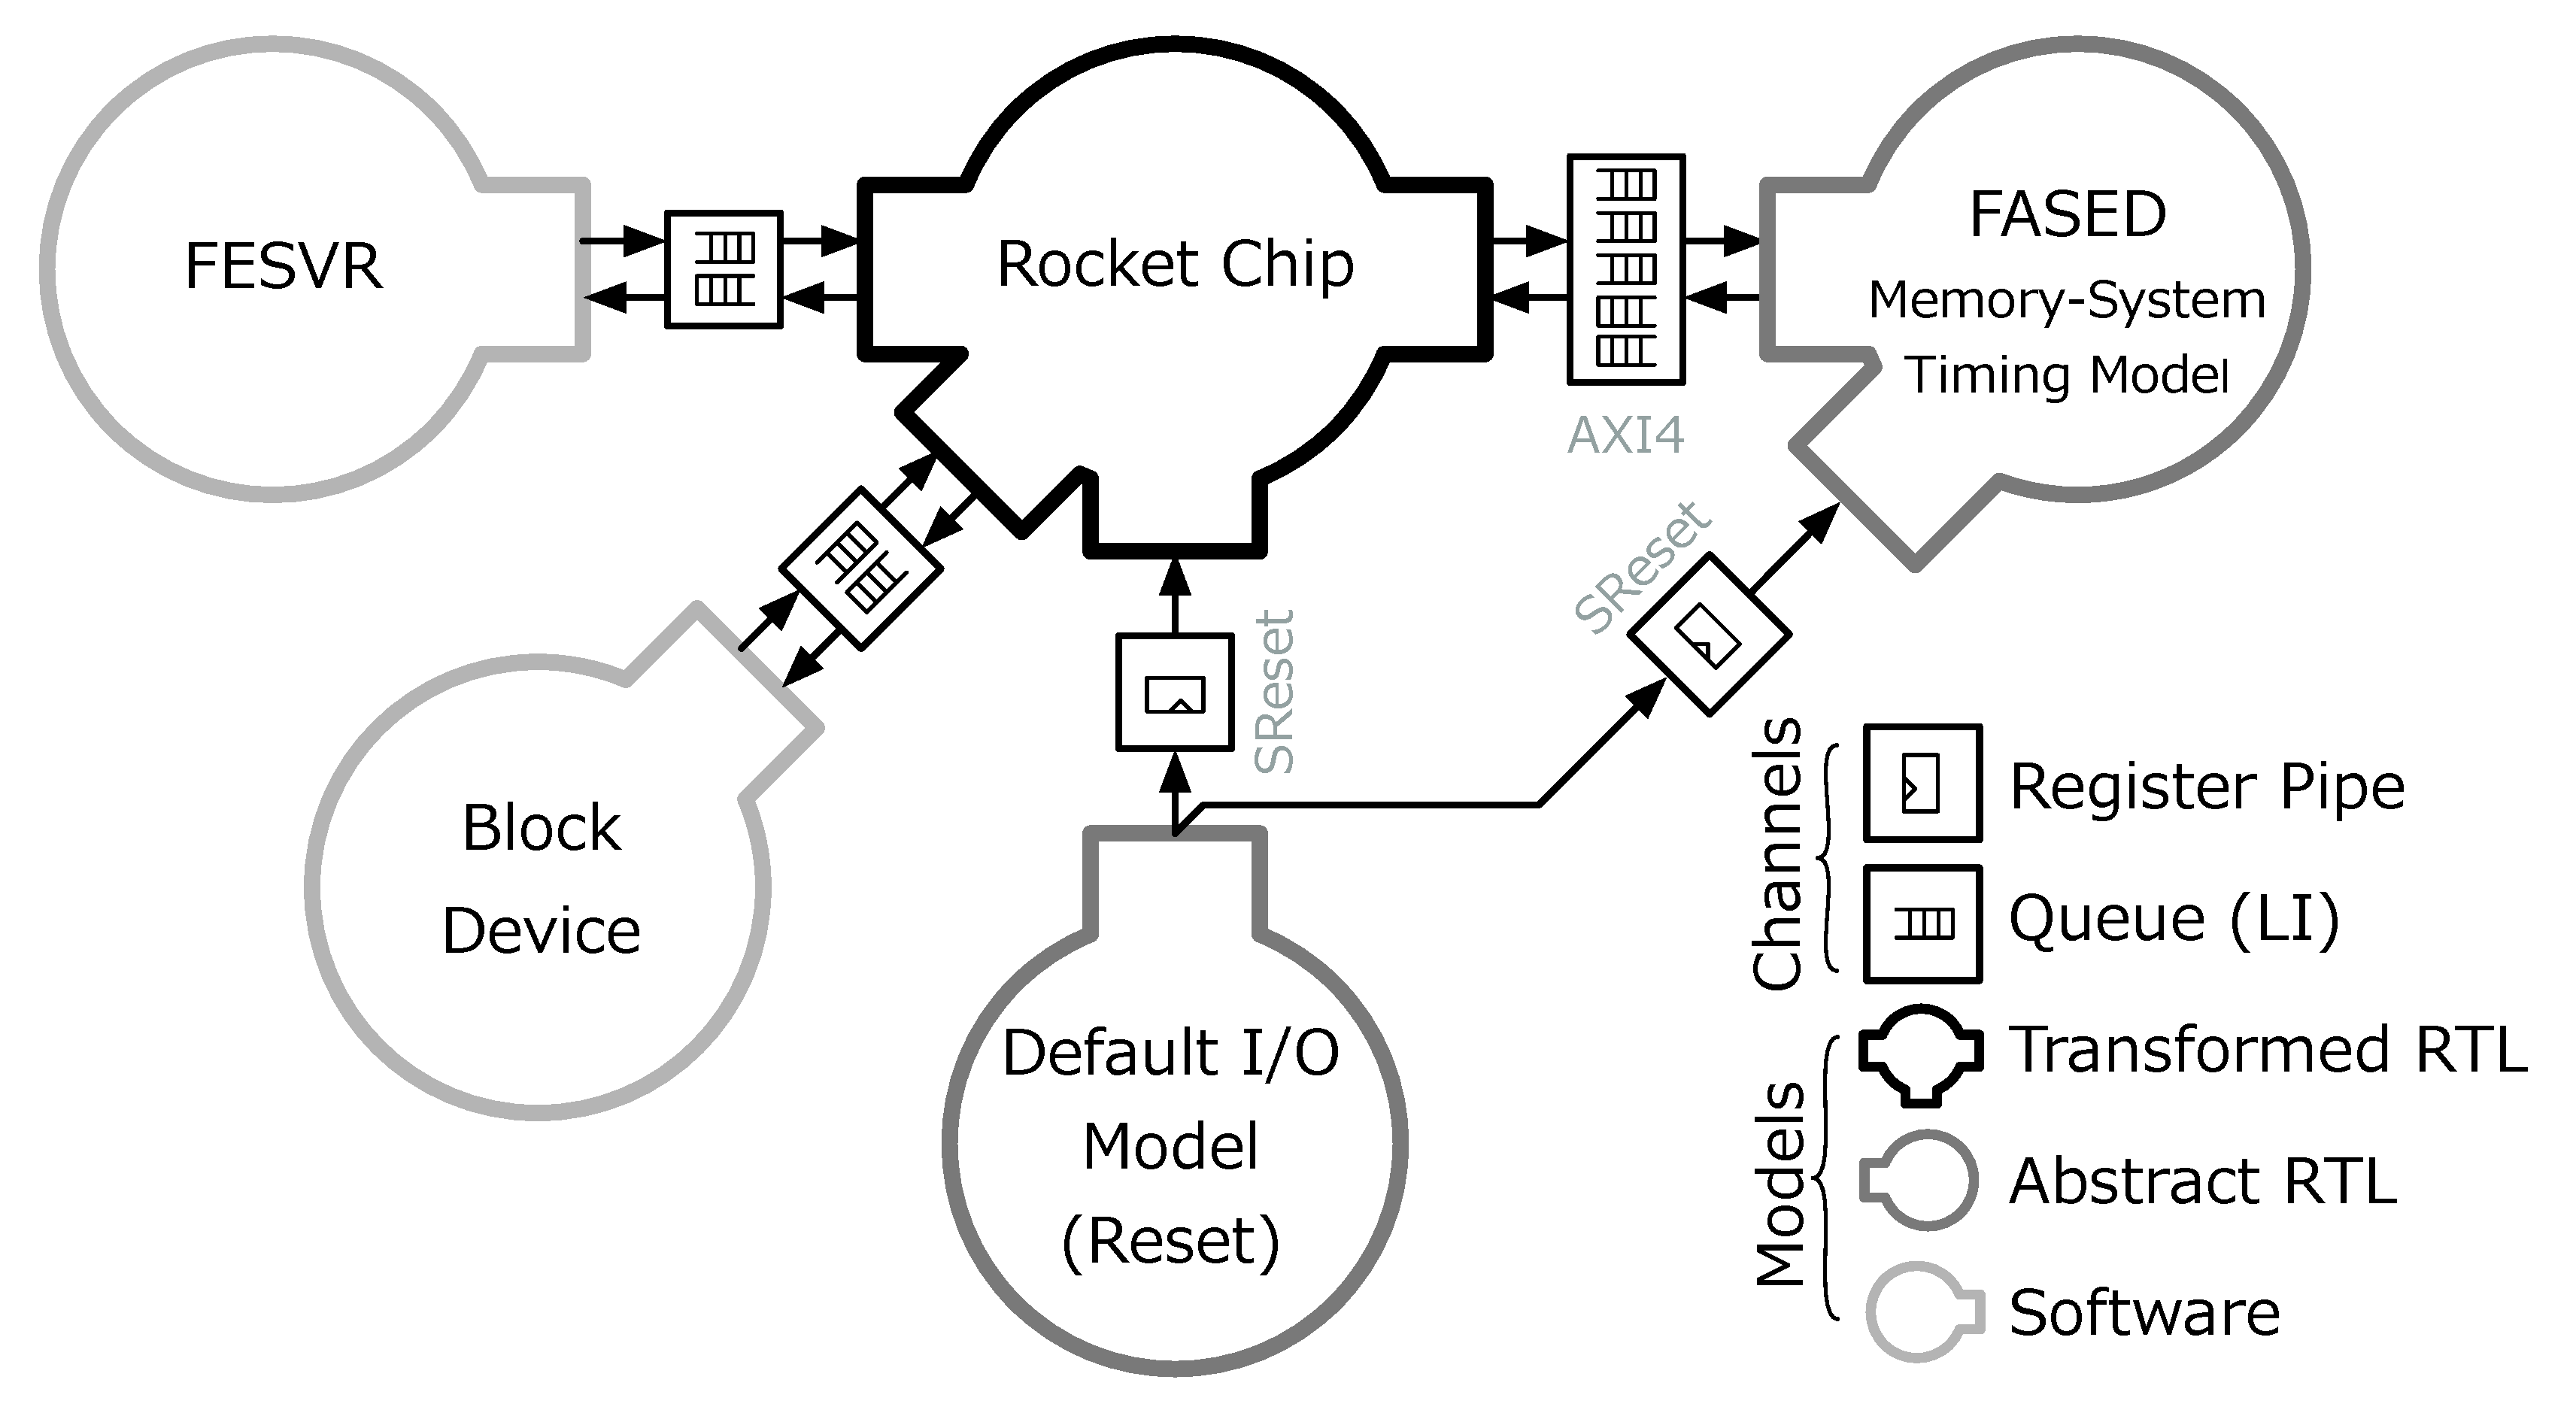
\includegraphics[width=\columnwidth]{figures/target-graph.pdf}
    % graffle2pdf -c target-graph midas-graphics/graffle/masters-target.graffle figures/target-graph.pdf
    \vspace{-0.10in}
    \caption{The graph of target designs studied in this paper.}
    \label{fig:default-target}
    \vspace{-0.15in}
\end{figure}

Once all of the simulation components have been generated, the simulation
interconnect is elaborated and bound to a single AXI4 slave port. All
memory-mapped simulation components are accessed through this
interface. Additionally, a crossbar is generated to arbitrate between components
that require FPGA-host DRAM. Ultimately, \SIMNAME emits a Verilog file and a
C++ header describing the simulator's memory map. To generate a bitstream, the
user instantiates the \SIMNAME-generated Verilog in a skeleton FPGA project
that exposes AXI4 interfaces to the FPGA's off-chip memory systems and
interconnect to the host CPU.

\subsection{Software Simulation Driver \& Software Models}
To control the simulator, the user writes a C++ program that links against the
\SIMNAME C++ libraries and the generated header. The \SIMNAME libraries implement
basic commands used to control simulation.  These commands are decomposed into
memory-mapped I/O issued over the simulation interconnect.  To complete
the simulator, the user links in software models into this program.

\section{Targets \& Hosts of This Paper}\label{sec:targetandhostmachines}

All target designs used in this work are tethered RISC-V processors with a
single-channel DRAM subsystem.  They share the target graph shown in
Figure~\ref{fig:default-target}. This graph comprises a Rocket-Chip-generated
transformed-RTL model that includes one to four Rocket pipelines with L1 caches
and a cache-coherence controller; software models for a UART~(not shown),
a block device, and the RISC-V front-end server
(FESVR, which provides BIOS-like functionality); and a \PNAME instance,
which connects to an AXI4 port presented by the processor.  All remaining I/O
of the transformed-RTL model, including reset, is bound to the default I/O
model.

\begin{figure}[t]
\vspace{-0.1in}
    \centering
    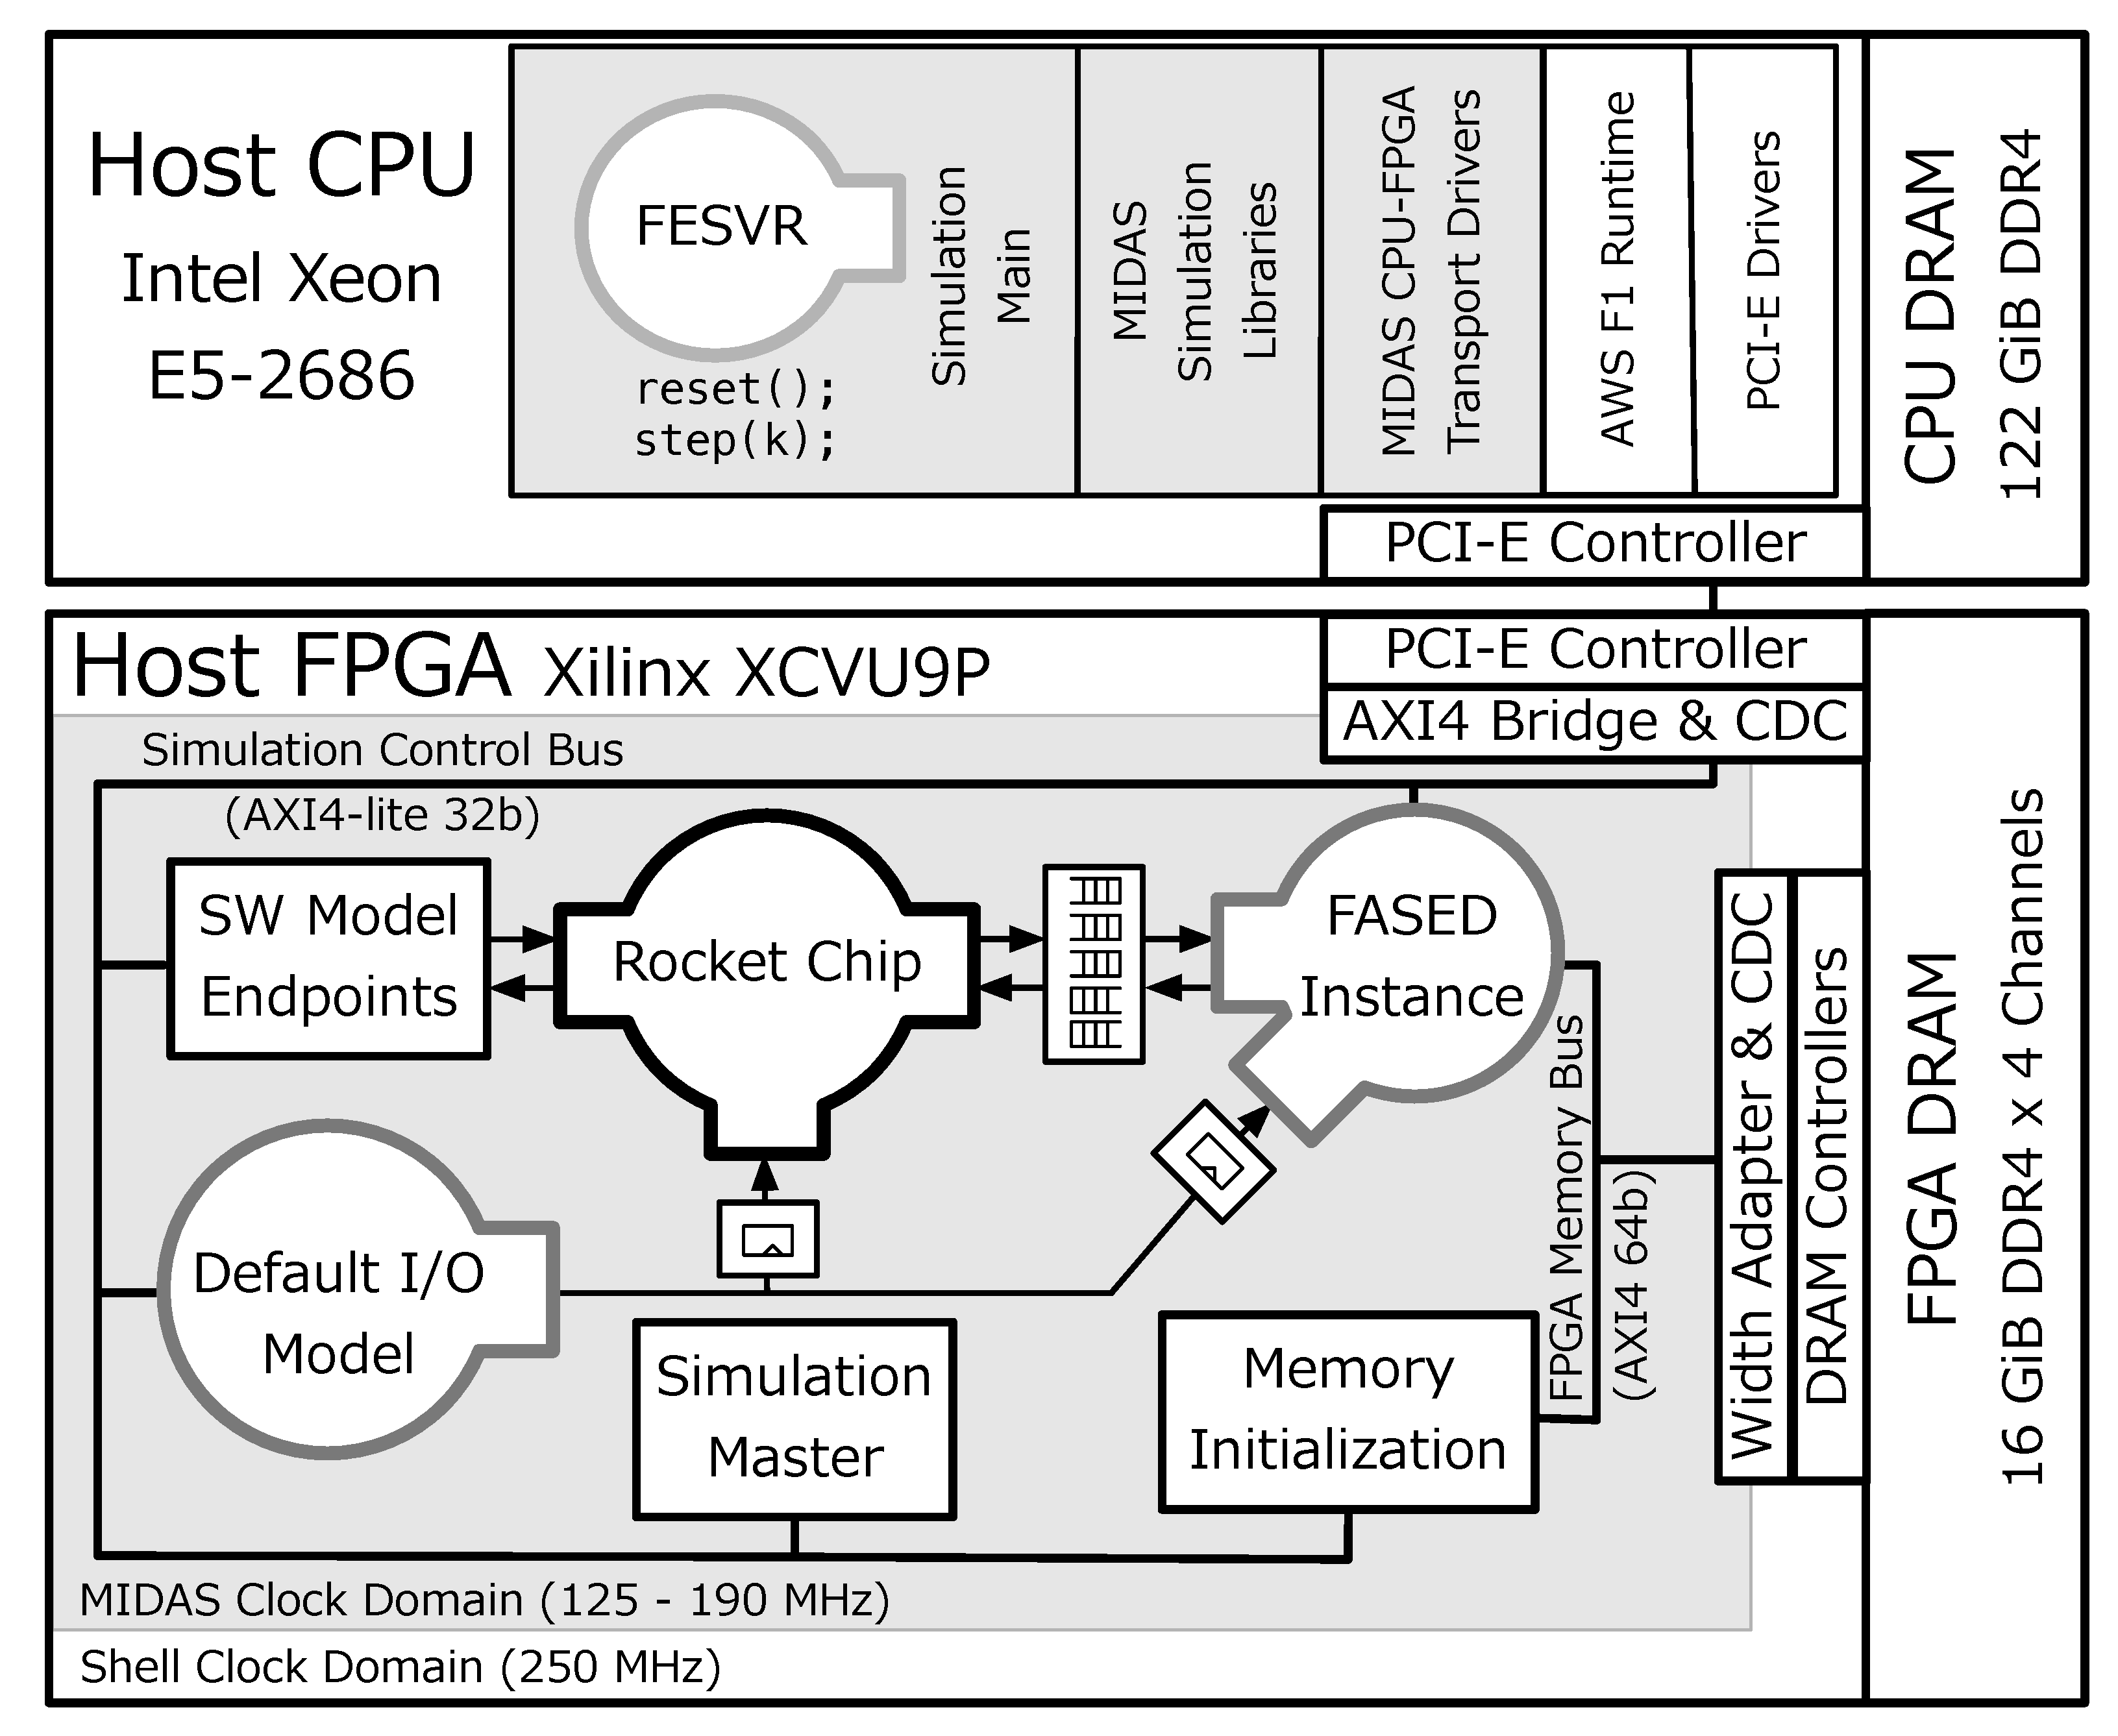
\includegraphics[width=\columnwidth]{figures/mapped-simulator.pdf}
    % graffle2pdf -c f1 midas-graphics/graffle/masters-target.graffle figures/mapped-simulator.pdf
    \vspace{-0.25in}
    \caption{The target mapped to an F1 host. The contribution of this work is
    the \PNAME instance, which replaces a crude latency-pipe model provided
    by the prior work.}
    \label{fig:mapped-simulator}
\vspace{-0.10in}
\end{figure}

While \SIMNAME supports other FPGA hosts, currently FireSim only has support for
Amazon EC2 F1 instances. F1's \texttt{f1.2xlarge} instances have a Xilinx
UltraScale+ XCVU9P\footnote{2.6 million logic cells, \wunits{346}{Mb} of
on-chip memory.}
attached to four \wunits{16}{GiB} channels of ECC-enabled DDR4 SDRAM.  FPGAs
are attached to a CPU with 8 hardware threads and \wunits{112}{GiB} of
DRAM. Figure~\ref{fig:mapped-simulator} shows the target mapped to an F1 host.
